\documentclass[12pt]{scrartcl}
\usepackage[utf8]{inputenc}
\usepackage[croatian]{babel}
\usepackage{amsmath,amssymb,amsthm}
\usepackage{marvosym}
%dodani paket za citat u uvodu
\usepackage{epigraph}

%dodano za potrebe naglaska na rijec
\usepackage[safe]{tipa}
%\usepackage{csquotes}
%\MakeOuterQuote{"}
\usepackage[unicode]{hyperref}
\usepackage{graphicx}
%\usepackage{tikz}
\usepackage{thmtools}
\declaretheorem{teorem}
\declaretheorem[style=definition,sibling=teorem,qed=$\square$]{definicija}



\begin{document}

\title{Qubic --- 3D križić-kružić}
\subtitle{Završni projekt - Multimedijski sustavi}
\author{Ivan Krcivoj, Antonela Bogdanić}
\date{Zagreb, \today}
\maketitle


\newpage

\tableofcontents

\newpage

\section{Uvod}
Jedna od najpoznatijih igara na svijetu zasigurno je križić-kružić, engl. \textit{tic-tac-toe}. Možda je upravo zbog svoje jednostavnosti pravila,
”opreme za igru” i strategije stekao takvu slavu među ljudima. Kao završni projekt iz kolegija Multimedijski sustavi odlučili smo se implementirati malo kompliciraniju varijantu ove popularne igre. 

Križić-kružić u tri dimenzije --- Qubic nije toliko popularan među igračima kao njegov prethodnik, no često je predmet proučavanja znanstvenika. Igra nudi mnoštvo strategija i posjeduje neka svojstva koja su veoma zanimljiva za proučavanje. Naša je ideja bila približiti "naizgled" tešku igru korisnicima i omogućiti igranje međusobno ili protiv računala.

Prije opisivanja igre, aplikacije za igranje i detalja samog programskog koda, iznijet ćemo kratku povijest Qubica. Parker Brothers predstavili su igru i krenuli prodavati set za igru davne 1964. 1972. prestavljaju novi moderniji izgled igre. Oba izdanja imala su naziv \textit{Parker Brother 3D Tic Tac Toe Game}. Set je uključivao prozirnu kocku za igranje i oznake igrača u bojama, no igra se može igrati i na papiru(Slika~\ref{fig:set} b)). Tako su se kasnije na tržištu pojavili i prazni papirnati predlošci za igranje Qubica(Slika~\ref{fig:set} a)). Paralelno uz popularizaciju igre za šire pučanstvo, razvijao se i interes znanstvenika koji su htjeli pronaći najbolju strategiju za garantiranu pobjedu prvog igrača. 


\begin{figure}[h]
	\centering
	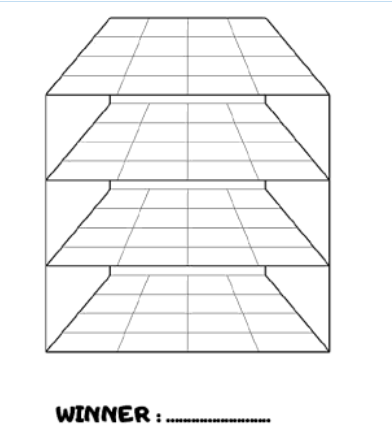
\includegraphics[height=40mm]{slika1a}
	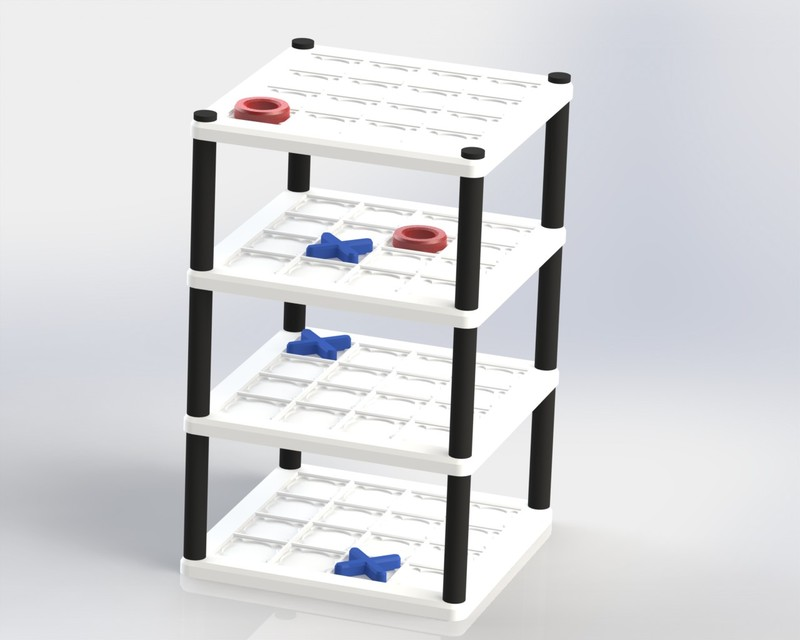
\includegraphics[height = 40mm]{slika1b}
	\caption{a) igra na papiru, b) igra na kocki}
	\label{fig:set}
\end{figure}

Ovu dokumentaciju smo podijelili na dva dijela. Prvi dio se odnosi na korisničku dokumentaciju, u kojoj ćemo opisati igru, navesti pravila igre i detaljno prikazati kako koristiti aplikaciju. U drugom dijelu bavit ćemo se detaljima implementacije, opisat ćemo pomoćne klase vezane uz logiku igre i objasniti dijelove koda. Nadamo se da će opisani dijelovi pomoći studentima prilikom unaprjeđenja našeg projekta, ali i korisnicima za što lakše korištenje. 




\part{Korisnička dokumentacija}
\section{Uvodno o igri}
Qubic je varijanta križić-kružića u tri dimenzije s ukupno 64 polja na koja dva igrača postavljaju znakove X ili O. Umjesto na ploči s 9 polja kao u ”klasičnoj ” varijanti igre, igrači u Qubicu postavljaju svoje oznake na kocki koja sadrži četiri horizontalne ploče sa 16 kvadratića, odnosno igra se na kocki dimenzija \texttt{4x4x4} kvadratića. Također, igru je moguće igrati i na kocki manjih dimenzija, konkretno \texttt{3x3x3}, tada kocka sadrži 27 polja za igru raspoređena na tri horizontalne ploče. 

Igra se unatoč trodimenzionalnosti može igrati i na papiru, no može se nabaviti i posebna kocka za igranje. Mi smo odlučili ploču za igru prikazati što jednostavnije kako bi korisnicima bilo lakše vizualizirati kocku. 

Pravila igre ne razlikuju se previše od križić-kružića na koji smo navikli. Za pobjedu je potrebno da jedan od igrača uspije složiti 4 (ili 3) svoja znaka u nizu. Igrač može na više načina složiti tzv. pobjedničke linije, engl. \emph{winning lines}. Igrač koji na bilo kojoj horizontalnoj ploči u retku, stupcu ili dijagonali složi svoje znakove pobijedio je. Nadalje, isto vrijedi i za vertikalne ravnine/ploče kocke. Posljednji način na koji je moguće pobijediti je tako da igrač složi znakove na neku od 4 glavne dijagonale kocke. 

Igrači naizmjenice igraju, tako da postavljaju svoje oznake na ploču, počevši od onog igrača koji ima oznaku X. U daljnjem ćemo radu prvog igrača, odnosno onoga
koji postavlja X označavati kraće kao X igrač ili samo X, analogno za igrača
O. Igra završava pobjedom nekog od igrača ili remijem ukoliko je cijela ploča
ispunjena, a nema pobjedničkih linija.

Nakon što smo opisali pravila, u sljedećim ćemo Vas točkama provesti kroz korištenje aplikacije i pokazati mogućnosti koje onda nudi. Nadamo se da ćemo primjerima i opisima olakšati korištenje navedene aplikacije i da će Vam igranje biti što ugodnije. 

\section{Pokretanje i početak igre}
Unutar repozitorija u kojem se nalazi ova dokumentacija, unutar podmape \emph{Qubic} možete pronaći datoteku naziva \emph{Qubic.pde}. 
Ona se pokreće koristeći \emph{Processing}(mi smo za pisanje i pokretanje koristili verziju \emph{4.0b2}.), a sama igra se pokreće pritiskom na gumb \texttt{Run}. 

\begin{figure}[ht]
	\centering
	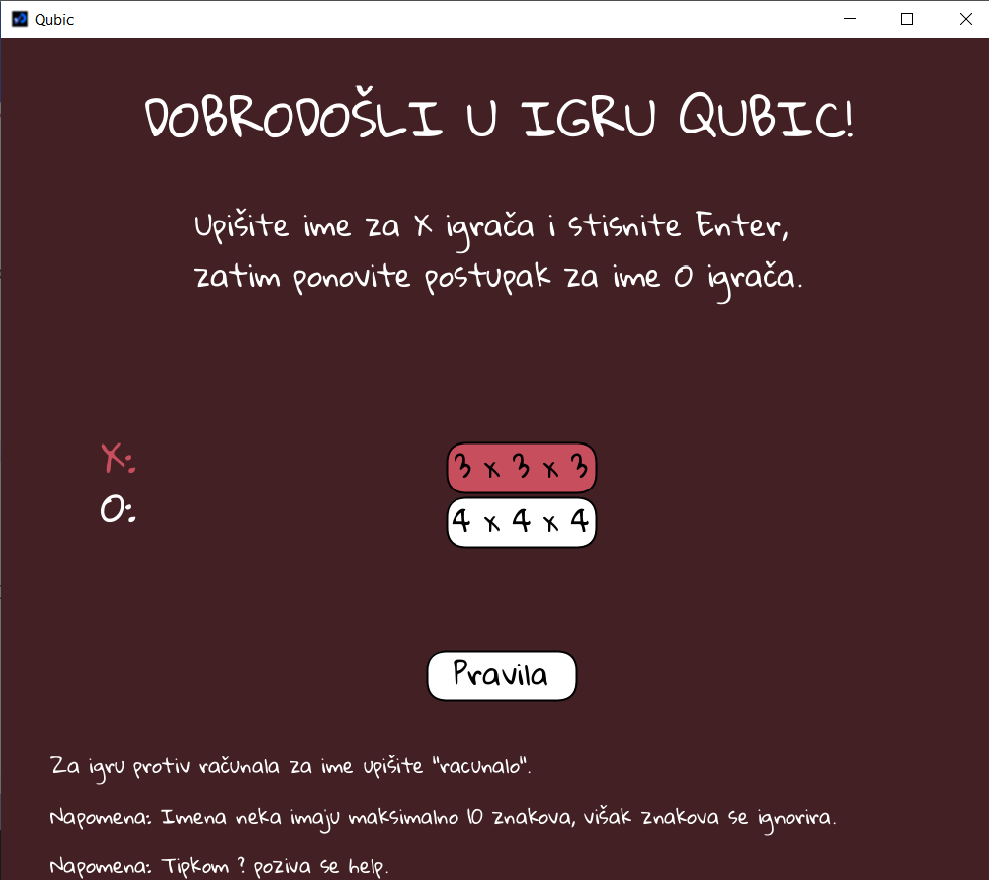
\includegraphics[scale=0.55]{pocetna.png}
	\caption{Početni zaslon aplikacije}
	\label{fig:poc}
\end{figure}

Nakon pokretanja na ekranu bi se trebao pojaviti prozor kao na Slici~\ref{fig:poc}. To je početni prozor aplikacije u kojem je potrebno odabrati vrstu igre i upisati imena igrača. Najprije se upisuje ime X igrača, vidimo da je on posebno označen na početku. Kada je korisnik unio željeno ime pritisne tipku \texttt{Enter}, tada je posebno označen O znak i po završetku pritiskom na \texttt{Enter} započinje igra.

Potrebno je napomenuti kako su imena igrača ograničena na sveukupno 10 znakova te da su neki simboli onemogućeni za korištenje jer služe kao poziv dodatnih funkcionalnosti u aplikaciji. Na primjer, nije moguće koristiti simbole: \texttt{\%,\$,\&,\#,?}. Također, sve dok nije upisano ime, pritiskom na \texttt{Enter} ništa se neće promijeniti.

Na početnom se zaslonu nalazi i mogućnost odabira vrste igre, korisnik može odabrati želi li igrati na ploči dimenzija \texttt{3x3x3} ili \texttt{4x4x4}. Kao zadana vrsta igre označena je igra na ploči \texttt{3x3x3}, a to lako promjeni klikom na željeni gumb. 

Također, na početnom zaslonu vidimo i gumb \texttt{Pravila}. Klikom na njega otvorit će se poseban prozor u kojem su ispisana pravila igre, ali o tome više u~\ref{sec:funk}. Napomena na dnu obavještava korisnike o mogućnosti korištenja \emph{help prozora} u kojem mogu pronaći popis dodatnih funkcionalnosti, kao i načina kako ih pokrenuti. Korištenje \emph{help} prozora klikom na tipku \texttt{?} omogućeno je tijekom cijelog korištenja aplikacije.

Iako je igra namijenjena za dva igrača, omogućili smo igranje protiv računala. Ako želite igrati protiv računala, potrebno je napisati \texttt{racunalo} kao ime igrača kojeg želite da igra računalo.

\newpage \section{Tijek igre}
Nakon unosa imena i odabira vrste igre pojavljuje se glavni zaslon aplikacije. Na njemu se vidi prikaz odabrane ploče kao i detalja same igre, kao na Slikama~\ref{fig:ploca3}~i~\ref{fig:ploca4}. Posebnom bojom označeno je ime igrača koji je na potezu, na početku smo rekli da je to igrač X. Svakim potezom promijenit će se oznaka igrača koji je na potezu, promijenit će se broj poteza koji piše na dnu prozora kao i stanje na ploči, primjer vidimo na Slici~\ref{fig:ploca4}.

\begin{figure}[h]
	\centering
	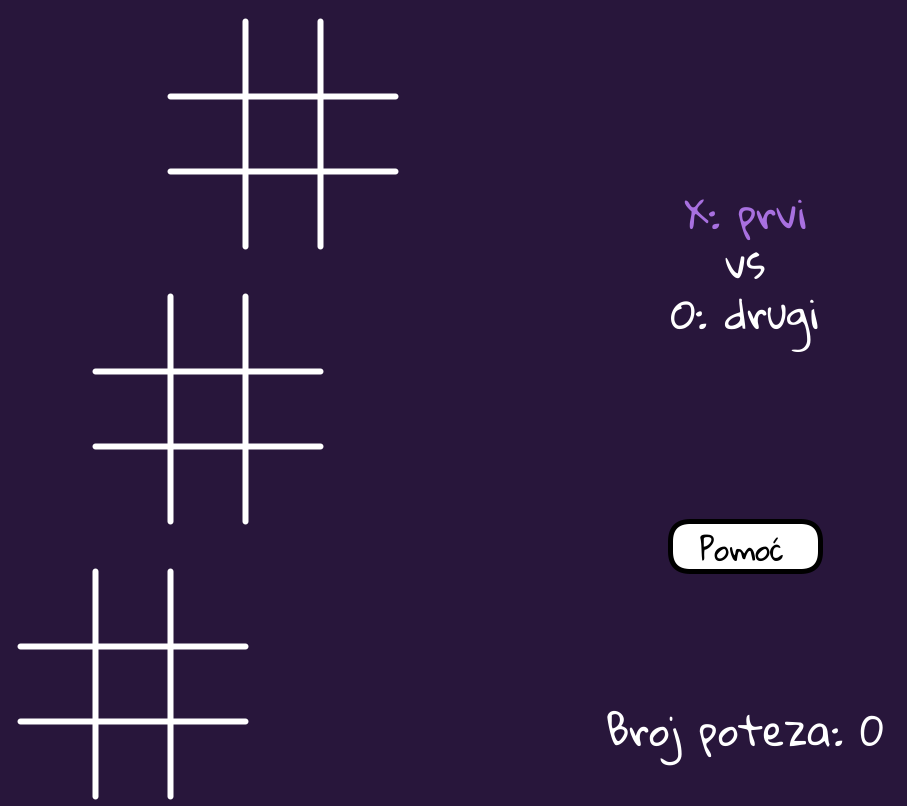
\includegraphics[scale=0.35]{ploca3.png}
	\caption{Ploča za igru \texttt{3x3x3}.}
	\label{fig:ploca3}
\end{figure}

\begin{figure}[h]
	\centering
	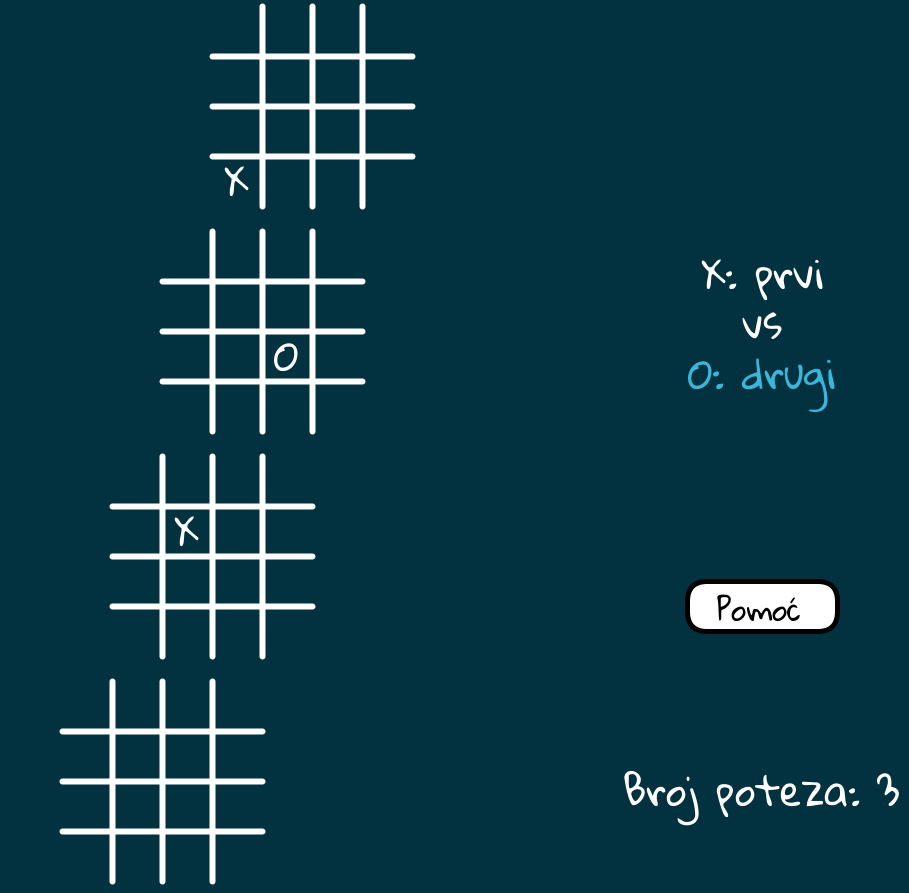
\includegraphics[scale=0.35]{ploca4.png}
	\caption{Ploča za igru \texttt{4x4x4}.}
	\label{fig:ploca4}
\end{figure}

Igrači klikom na željeno polje na ploči odigraju svoj potez. Potez je ispravan kada je igrač kliknuo unutar nekog polja na ploči i pritom je to polje neodigrano, odnosno prazno. Zvuk koji se pritom čuje moguće je isključiti pritiskom na tipku \texttt{\#}, ali o tome u~\ref{sec:funk}. Ukoliko je potrez neispravan, prikazat će se odgovarajuća poruka kao na Slici~\ref{fig:poruka}.

\begin{figure}[h]
	\centering
	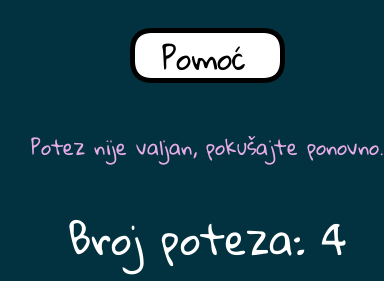
\includegraphics[scale=0.5]{poruka.png}
	\caption{Poruka o neispravnom potezu.}
	\label{fig:poruka}
\end{figure}

Na tom se prozoru još nalazi i gumb \texttt{Pomoć}. On služi kao pomoć igračima prilikom igranja igre. S obzirom na složenost traženja najboljeg poteza zbog velikog broja mogućnosti, izračunavanje poteza može potrajati. Ako je potez izračunat, prelaskom miša po gumbu \texttt{Pomoć} gumb će se pobojati posebnom bojom koja ovisi o odabiru teme(više u~\ref{sec:funk}), kao na Slici~\ref{fig:pom} a). U slučaju da se potez još računa prelaskom miša po gumbu \texttt{Pomoć} on će izgledati kao na Slici~\ref{fig:pom} b), posebno naglašen sivom bojom uz prateću poruku.

\begin{figure}[h]
	\centering
	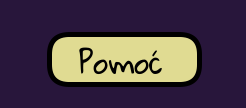
\includegraphics[height=2cm]{pomoc.png}
	
\includegraphics[height=2cm]{pomoc-racunanje.png}
	\caption{Primjer prelaska miša preko gumba: \newline a) kada je potez izračunat, b) kada računanje još traje}
	\label{fig:pom}
\end{figure}

Kada je potez izračunat, klikom na gumb \texttt{Pomoć} na ploči se posebnom bojom označi potez koji računalo predlaže kao najbolji potez. Primjer možete vidjeti na Slici~\ref{fig:hint}.

Igra s računalom odvija se na isti način kao u slučaju dva igrača. Jedina je razlika što dok je računalo na potezu korisnik ne može igrati poteze, nego mora pričekati da računalo odigra svoj potez. 

\begin{figure}[ht]
	\centering
	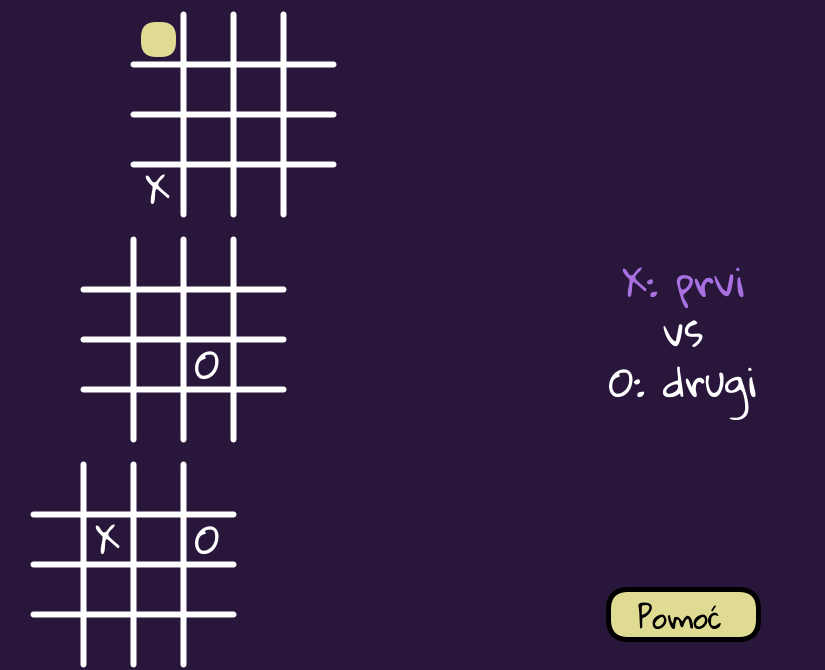
\includegraphics[scale=0.4]{hint.png}
	\caption{Prikaz hinta na ploči.}
	\label{fig:hint}
\end{figure}

\newpage \section{Kraj igre}\label{sec:kraj}
Igra završava pobjedom nekog igrača nakon što složi tzv. pobjedničku liniju ili remijem ako je cijela ploča popunjena. Završni zaslon u pozadini ima oznaku igrača koji je pobijedio ili zajedničkih oznaka u slučaju remija, primjer na Slici~\ref{fig:kraj}. Ispisuje se i pripadna poruka o pobjedi igrača ili remija u određenom broju poteza. Izgled pozadine osim o pobjedi X ili O igrača ovisi i o temi aplikacije koju je korisnik odabrao, a ako je korisnik omogućio zvuk čut će se i prigodni zvuk pobjede. Rezultati igre spremaju se automatski u datoteku rezultata. Omogućen je povratak na početni zaslon pritiskom na tipku \texttt{SPACE}. 

\begin{figure}[h]
	\centering
	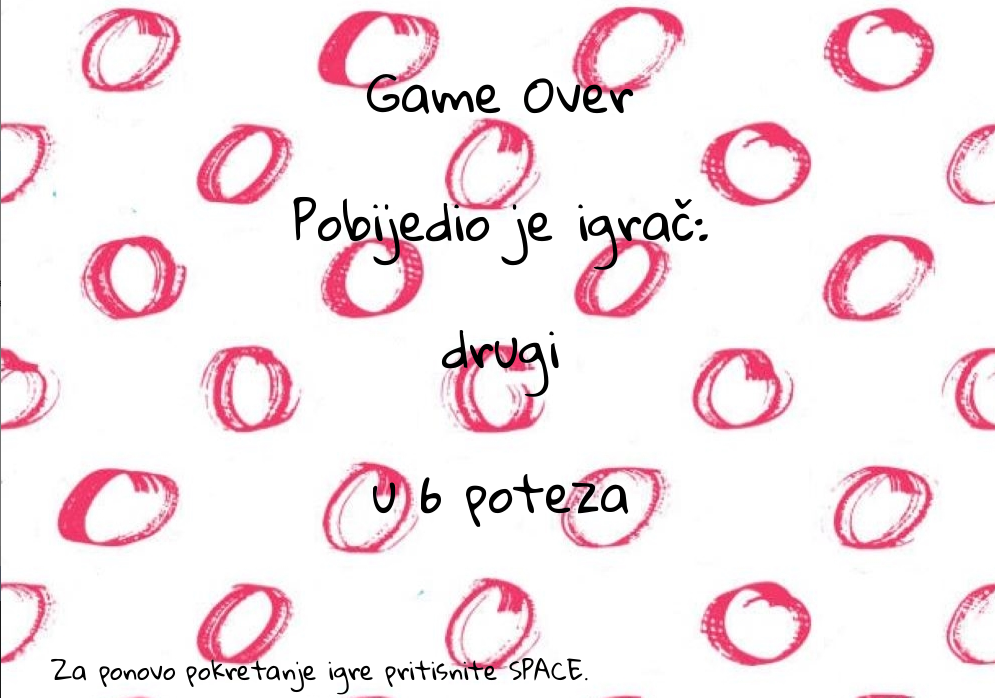
\includegraphics[scale=0.25]{kraj.png}
	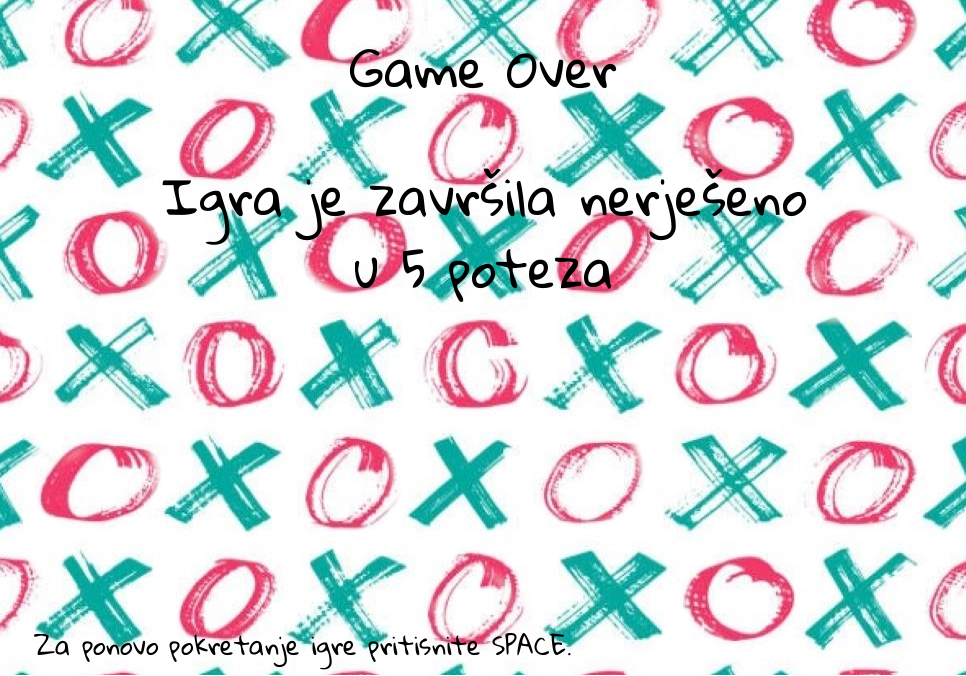
\includegraphics[scale=0.25]{remi.png}
	\caption{Primjer završnog zaslona u slučaju: a) pobjede O igrača b) remija}
	\label{fig:kraj}
\end{figure}


\section{Dodatne funkcionalnosti}\label{sec:funk}

U ovoj ćemo točki objasniti nekoliko dodatnih funkcionalnosti i objasniti kako se koriste.

\begin{figure}[h]
	\centering
	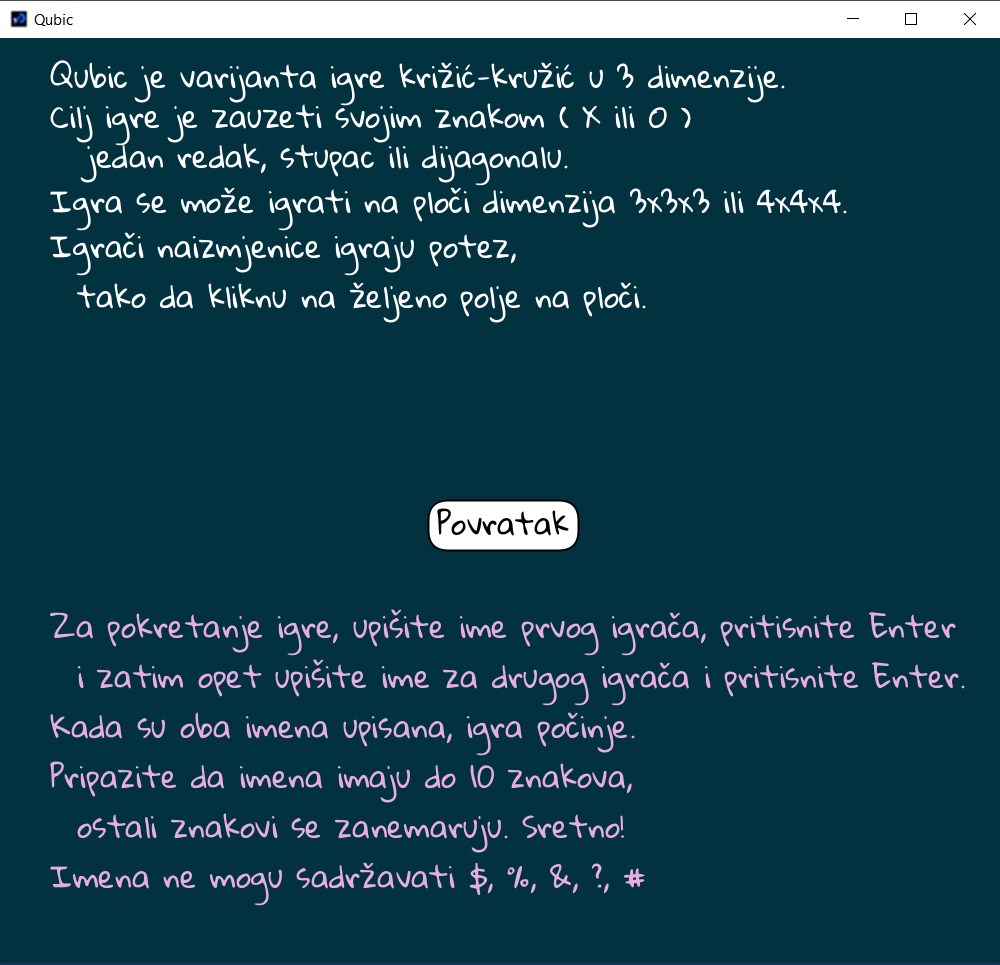
\includegraphics[scale=0.3]{pravila.png}
	\caption{Pravila igre}
	\label{fig:pravila}
\end{figure}


 Za početak prisjetimo se gumba \texttt{Pravila} koji se nalazio na početnom zaslonu aplikacije, Slika~\ref{fig:poc}. Klikom na njega prikazuje se prozor kao na Slici~\ref{fig:pravila}. Kratko su ispisana pravila igre kao i upute o pokretanju igre uz dodatne napomene. Klikom na gumb \texttt{Povratak} vraćamo se na početni zaslon. Prelazak mišem preko oba gumba posebnom će bojom označiti gumb. 


Sljedeća funkcionalnost koja je omogućena je pozivanje \emph{help} izbornika. On se poziva klikom na tipku \texttt{?}. Na Slici~\ref{fig:help} možete vidjeti kako izgleda taj zaslon. Osim što vidimo opise i načine korištenja svih funkcionalnosti, vidimo i prikaz tema koje je moguće koristiti u aplikaciji. Teme su konkretno palete boja koje se koriste u aplikaciji. Mi smo omogućili 3 različite palete --- teme, a one se lako mijenjaju pritiskom na tipke: \texttt{\$,\%,\&}.

\begin{figure}[h]
	\centering
	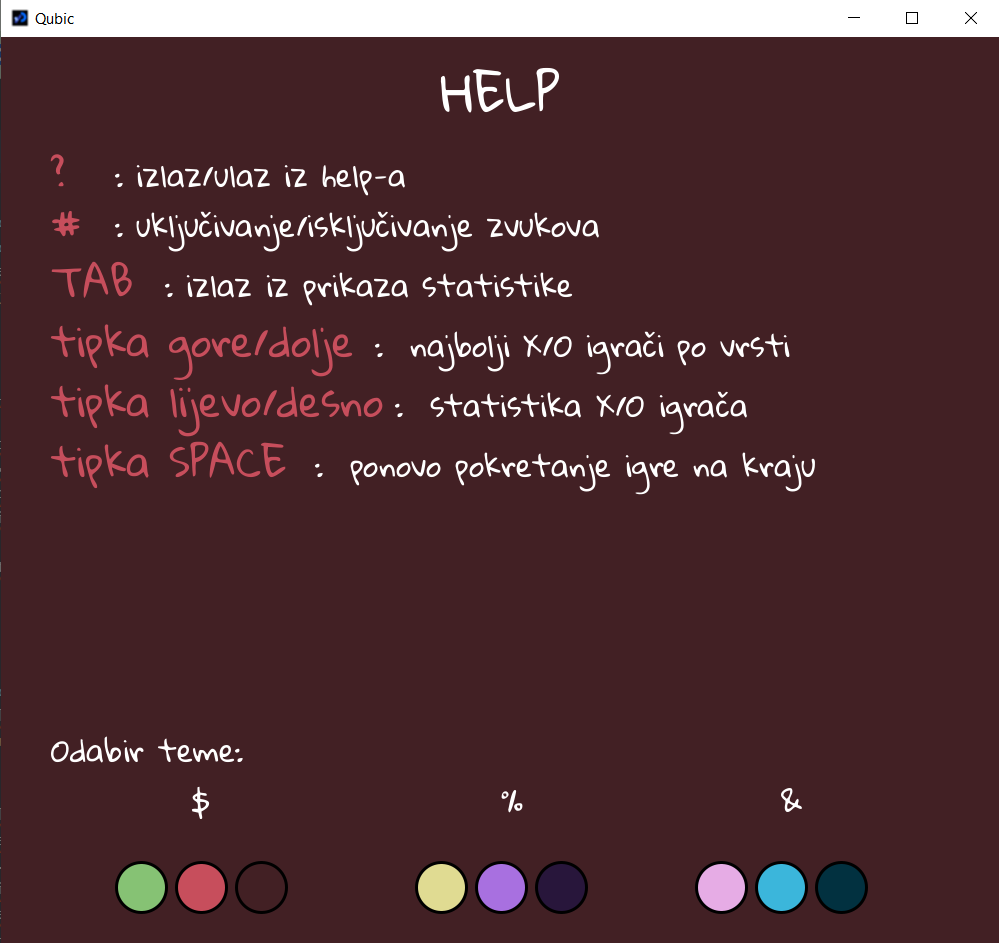
\includegraphics[scale=0.5]{help.png}
	\caption{\emph{Help} izbornik}
	\label{fig:help}
\end{figure}

Opišimo redom preostale funkcionalnosti koje vidimo u \emph{help} izborniku. Tipkom \texttt{\#} uključujemo ili isključujemo zvukove u aplikaciji, a to su zvukovi igranja poteza i zvuk na kraju igre. 

Sljedeća funkcionalnost koja je omogućena, i već spomenuta u točki~\ref{sec:kraj}, je povratak na početni zaslon tipkom \texttt{SPACE}. Taj je povratak omogućen samo ukoliko smo na završnom zaslonu, odnosno završili s igrom. \newpage
\begin{figure}[h]
	\centering
	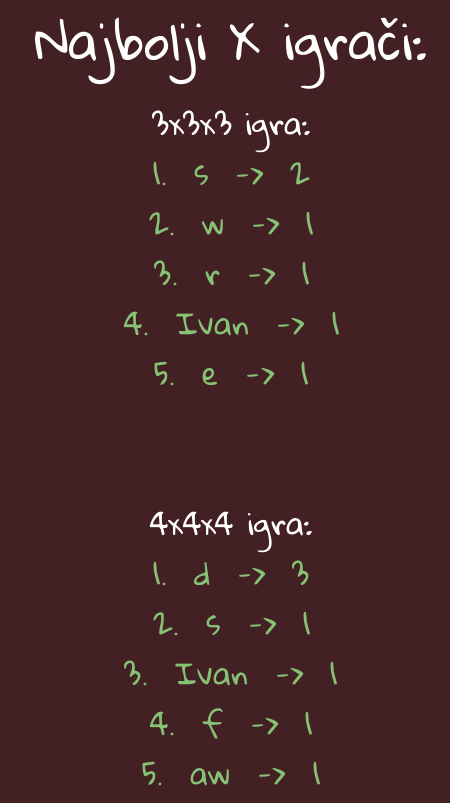
\includegraphics[scale=0.4]{statX.png}
	\caption{Prikaz 5 najboljih X igrača po vrsti igre}
	\label{fig:statX}
\end{figure}

\begin{figure}[h]
	\centering
	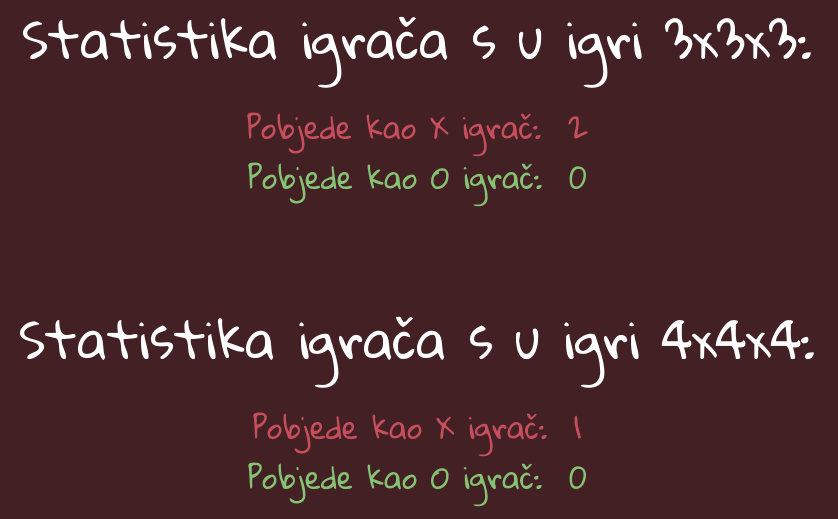
\includegraphics[scale=0.4]{statIgrac.png}
	\caption{Prikaz statistike trenutnog igrača}
	\label{fig:stat}
\end{figure}
Zadnja funkcionalnost koju je preostalo opisati je prikaz statistike. Postoji više različitih prikaza statistike koje je moguće pregledati u aplikaciji, a svi se pozivaju klikom na tipke strelica. Strelica gore poziva ispis pet najboljih X igrača ovisno o vrsti igre(Slika~\ref{fig:statX}, dok strelica dolje prikazuje 5 najboljih O igrača. Strelica lijevo poziva prikaz osobne statistike X igrača koji trenutno igra Qubic, dok strelica desno prikazuje osobne rezultate trenutnog O igrača, primjer na Slici~\ref{fig:stat}. Ukoliko se osobna statistika poziva na početku igre i imena igrača još nisu upisana, tada se ispiše poruka: \texttt{Upišite ime igrača pa pokušajte ponovo vidjeti statistiku!}. Izlaz iz prikaza statistike događa se pritiskom na tipku \texttt{TAB}.


\part{Tehnička dokumentacija}
\section{Opis projekta}
U ovom ćemo dijelu dokumentacije detaljno objasniti programski kod i detalje implementacije kako bi kolegama koji će nadograđivati našu aplikaciju što više olakšali posao. Za početak objasnit ćemo okruženje u kojem smo stvarali kod i navesti materijale koji su dio projekta. 

Sve materijale možete pronaći na:~\url{https://github.com/antonelab/Qubic-Processing}. U dokumentu \emph{Opis projekta.docx} nalaze se detalji našeg stvaranja projekta, poput podjele poslova, tijeka rada i popis poslova koje smatramo da još treba obaviti. Datoteka naziva \emph{Qubic.pdf} je upravo dokumentacija koju čitate, a materijali za stvaranje \texttt{.pdf} datoteke možete pronaći u podmapi \emph{dokumentacija}.

Programski kod u kojem smo implementirali igru i napravili aplikaciju nalazi se u podmapi \emph{Qubic}. Unutar nje nalazi se \emph{Qubic.pde} u kojem se nalazi glavni dio programskog koda, a koji se otvara i pokreće koristeći \emph{Processing}(mi smo koristili verziju \emph{4.0b2}). U podmapi \emph{code} nalaze se pomoćne klase u Javi i datoteka \emph{Qubic.jar}, dok se u podmapi \emph{data} nalaze se potrebni materijali za rad aplikacije poput fonta, zvuka i pozadina. 

Kao pomoć pri pisanju projekta, konkretno klasa u Javi, koristili smo \emph{NetBeans} u kojem smo stvorili projekt i provjeravali dijelove koda. Također, htjeli bi napomenuti da treba biti oprezan pri spajanju pomoćnih klasa s \texttt{.pde} datotekom, mi smo to uspijeli postići na način na koji je programski kod sada organiziran. Zbog toga smo dodali liniju \texttt{import qubic.*;}. Odgovarajuću \texttt{.jar} datoteku dobili smo upravo koristeći \emph{NetBeans}.

Prije objašnjavanja koda potrebno je ispisati dodatne biblioteke koje smo koristili u \emph{Processingu} prilikom izrade aplikacije. Potrebno je instalirati i \emph{importati} biblioteku \texttt{Sound} i \texttt{Minim} koje nam služe za korištenje zvukova. Također, zbog dodatnih \emph{Javinih} funkcija koje koristimo prilikom spremanja rezultata u datoteku potrebno je \emph{importati} i \texttt{java.io.FileWriter}.


\section{Logika igre}
Logika igre većinski je smještena unutar pomoćnih klasa u podmapi \emph{code}. 
Ukratko ćemo proći kroz dijelove datoteka obzirom na to da su oni dobro komentirani, no bitno je reći gdje se što nalazi kako bi se mogli lakše snaći u datotekama.

\subsection{\texttt{Cube}, \texttt{Cube3} i \texttt{Cube4}}
\texttt{Cube} je \textit{interface} koji predstavlja ploču za igru. U njoj se nalaze važne funkcije koje su potrebne za rad s kockom, a njih ćemo implementirati u klasama \texttt{Cube3} i \texttt{Cube4}. \texttt{Cube3} predstavlja kocku \texttt{3x3x3}, a klasa \texttt{Cube4} kocku \texttt{4x4x4}. Obzirom na to da su klase međusobno jako slične, mi ćemo malo detaljnije opisati \texttt{Cube4}. 

Redom, \texttt{Cube4} je konstruktor kocke i stvara praznu kocku tako što poziva \texttt{clear}. Funkcija \texttt{clear} postavlja sva polja ploče na ’ ’ što predstavlja da je to polje prazno i postavlja \texttt{mNumber} na 0 obzirom da nema oznaka na polju na početku igre. Kako bi mogli znati što se nalazi na određenom polju
kocke funkciji \texttt{value} dajemo 3 integera, odnosno oznaku pozicije. Intovi i, j, k su brojevi od 0 to 3, npr. trojka (1,2,2) predstavlja poziciju na kocku: prvi nivo (druga ploha od gore), drugi redak (na toj plohi) i drugi stupac (drugi stupac gledajući s lijeva na desno), za primjer pogledati Sliku~\ref{fig:ploca4} i poziciju O.


Funkcija \texttt{result} vraća broj koji predstavlja pobjedu, remi ili trajanje igre. Prilikom provjere pobjede nekog od igrača zovemo \texttt{winning\_line} koja nam vraća oznaku pobjedničkog igrača. Ako pobjeđuje X vrijednost završnog stanja je 500, a za O -500, ali ako funkcija nije vratila oznaku X ili O, a nema slobodnih polja na kocki jer je \texttt{mNumber} maksimalan, onda je završno stanje neriješeno i vrijednost 0. Funkcija \texttt{winning\_line} sadrži petlje koje prolaze po svim mogućim pobjedničkim linijama (ukupno 76) i provjeravaju postoje li 4 ista znaka u toj liniji te ako da vrate oznaku kojoj pripadaju.

Slijede četiri jednostavne funkcije, a to su redom: \texttt{generate\_moves} koja prolazi cijelom kockom i provjerava je li polje prazno (tj. ’ ’). Ako je polje prazno, moguće je odigrati potez na toj poziciji pa stvorimo \texttt{Move} objekt koji dodamo u vektor koji pohranjuje sve moguće poteze na kocki. Move klasa opisana je~\ref{subsec:m}. 

Zatim slijedi funkcija \texttt{isValid} koja provjera je li potez valjan. Potez je valjan ako su sve varijable članice postavljene na 0,1,2 ili 3 te je polje (i, j, k) na ploči prazno tj. ’ ’. Nadalje, funkcija \texttt{play} koja odigra potez move s oznakom igrača tako što najprije provjeri je li potez valjan s funkcijom \texttt{isValid}.


Ako je potez valjan treba ”odigrati” potez stavljajući oznaku igrača na poziciju na ploči koja odgovara potezu. Vraća se \emph{true} ili \emph{false} vrijednost ovisno o tome
je li potez bio valjan. Osim što možemo odigrati potez, možemo ga i ”vratiti”, odnosno u samom algoritmu nam kasnije treba \emph{undo} poteza pa to radi upravo funkcija \texttt{unPlay}. Način na koji se to izvodi je da vrati oznaku praznog polja ’ ’ na mjesto koje odgovara potezu \texttt{move} i broj odigranih poteza \texttt{mNumber} smanji se za jedan.

\subsection{\texttt{Move}}\label{subsec:m}
\texttt{Move} je klasa koja predstavlja potez. Kako se igranje igra odvija u tri dimenzije, \texttt{Move} ima tri koordinate \texttt{mLevel}, \texttt{mRow}, \texttt{mColumn}, koje predstavljaju razinu, red i stupac. Objekt klase \texttt{Move} možemo konstruirati na tri načina. Defaultni konstruktor sve vrijednosti postavlja na nulu, zatim imamo konstruktor koji prima redom vrijednosti razine, retka i stupca. Posljednji konstruktor prima \emph{string} koji se treba sastojati od tri broja koji su međusobno odvojeni zarezom. 

Pomoću odgovarajućeg \emph{gettera} možemo pročitati željenu koordinatu poteza. \emph{Setteri} ne postoje jer nije predviđeno da se vrijednosti komponenti mijenjaju.

Postoje nadjačane metode \texttt{equals} i \texttt{toString} koje uspoređuju dva poteza, odnosno pretvaraju potez u \emph{string} kako bi ga bilo moguće ispisati.

\subsection{\texttt{Pair}}
Klasa \texttt{Pair} je parametrizirana klasa koja se sastoji od dva atributa koji mogu biti različitih tipova. Koristimo ju kada želimo omogućiti funkciji da vrati dvije vrijednosti.

\subsection{\texttt{Player}}
Igrača predstavlja klasa \texttt{Player} koja pamti ime i simbol igrača. Simbol kojeg igrač koristi postavlja se u konstruktoru i kasnije se ne može mijenjati.

\texttt{minMax} je funkcija koja predstavlja stablo odluke s alfa-beta podrezivanjem. Funkcija vraća par koji se sastoji od heurističke vrijednosti najpovoljnijeg poteza te koji je najpovoljniji potez. Za to izračunavanje funkciji su potrebni redom: trenutno stanje na kocki, niz dopustivih poteza, oznaka igrača na potezu, vrijednost parametara alfa i beta te maksimalnu dubinu. Kako je broj mogućnosti velik koristimo alfa-beta podrezivanje kako ne bi morali provjeravati situacije u kojima znamo da ne možemo dobiti bolje rješenje. Međutim, kako broj stanja koji trebamo provjeriti i dalje može biti prevelik koristimo potragu do zadane dubine kako igra ne bi predugo trajala.

Funkcija \texttt{hint} prima stanje kocke i pomoću funkcije \texttt{minMax} računa optimalni potez. Kako izračunavanje pomoći može potrajati izvodit ćemo ga u zasebnoj dretvi pa nakon što izračunamo hint provjeravamo je li u međuvremenu korisnik odigrao sljedeći potez. U tom slučaju \emph{hint} nam više nije koristan pa ga odbacujemo podizanjem \texttt{interrupt} izuzetka. Ukoliko sljedeći potez nije odigran, hint je valjan pa ga prosljeđujemo dalje kao povratnu vrijednost.

\subsection{\texttt{Hint}}
\texttt{Hint} je klasa koja implementira sučelje \texttt{Runnable} i služi za računanje \emph{hinta} u posebnoj dretvi.

\subsection{\texttt{QubicGame}}
\texttt{QubicGame} je klasa u kojoj je implementirana logika igre. U konstruktoru prima tip igre i dva igrača koji međusobno igraju. Tip igre je broj 3 ili 4 i određuje koje će biti dimenzije kocke za igru. 

Funkcija \texttt{play} je najvažnija funkcija u ovom dijelu izlaganja. Pozivanjem te funkcije započinje izvršavanje same igre. Sastoji se od petlje koja čeka idući potez sve dok ne dođe do završnog stanja igre. Kada se odigra novi potez naprave se sve potrebne promjene kako bi igra funkcionirala. Po dolasku u završno stanje igre određuje se tko je pobijedio te time funkcija završava svoje izvođenje.

Kako čekanje na potez traje, radi izbjegavanja blokiranja igre, klasa \texttt{QubicGame} implementira sučelje \texttt{Runnable}. Nadjačana funkcija \texttt{run} omogućava da se funkcija \texttt{play} izvodi u zasebnoj dretvi.

\section{\texttt{Qubic.pde}}
U ovoj se datoteci nalaze dijelovi koda koji povezuju logiku igre s aplikacijom i određuju izgled i funkcionalnosti aplikacije. 
Obzirom na količinu i raspored programskog koda odlučili smo ovaj dio opisati na način da objasnimo globalne varijable,a zatim svaku pojedinu funkciju. 

\subsection{Globalne varijable}\label{subsec:var}
Zbog velikog broja globalnih varijabli koje koristimo prikazat ćemo ih sažeto i pregledno u nastavku, dok ćemo u kasnijim točkama spomenuti na kojim ih mjestima koristimo. 
\begin{itemize}
    \item \texttt{type} - predstavlja vrstu igre, može biti 3 ili 4
    \item \texttt{showHint} - pomoćna varijabla koja određuje treba li se prikazati/iscrtati \emph{hint} na ploči
    \item \texttt{written} - pomoćna varijabla koja služi kako bi se samo jednom upisali rezultati igre u statistiku
    \item \texttt{mess} - pomoćna varijabla koja govori imamo li poruku o grešci koju treba prikazati na glavnom prozoru
    \item \texttt{name} - globalna varijabla koja simbolizira stanje u kojem je naša aplikacija, zadana vrijednost je 1 i označava da X igrač unosi svoje ime, 2 označava da ime postavlja O igrač, a ako je vrijednost 0 to znači da su oba igrača unijeli svoje ime
    \item \texttt{info} - globalna varijabla koja govori o tome treba li iscrtati zaslon s pravilima, ako je 1 zaslon se iscrtava
    \item \texttt{help} - globalna varijabla koja govori o tome treba li iscrtati zaslon s naredbama, ako je 1 zaslon se iscrtava
    \item \texttt{stat} - globalna varijabla koja služi za prikazivanje statistike, ovisno o vrijednosti prikazuju se različite vrste statistika, zadana vrijednost je 0 jer se statistika ne prikazuje, ako je 1 ili 2 prikazuju se najbolji igrači X ili 0, ako je 3 prikazuju se osobne statistike
    \item \texttt{mute} - pomoćna varijabla koja služi za isključivanje ili uključivanje zvuka, ako je 0 zvuk je omogućen
    \item \texttt{newGame} - pomoćna varijabla koja služi na kraju igre kako bi znali trebamo li ponovo iscrtati početni zaslon, zadana vrijednost je 0, a kada je 1 iscrtat ćemo ponovo početni zaslon
    \item[$\blacksquare$] \texttt{player1} i \texttt{player2} - spremamo objekte tipa \texttt{Player} koji predstavljaju naše igrače
    \item[$\blacksquare$] \texttt{game} - predstavlja objekt \texttt{QubicGame} koji predstavlja igru 
    \item[$\blacksquare$] \texttt{gameThread} - dretva u kojoj se čeka da korisnik odigra potez
    \item[$\blacksquare$] \texttt{font} - spremamo font koji koristimo u cijeloj aplikaciji
    \item[$\blacksquare$] \texttt{move\_sound} i \texttt{win\_sound} - varijable koje spremaju imena datoteka zvukova 
    \item[$\blacksquare$] \texttt{minim, minim2} i \texttt{audio\_win, audio} - varijable potrebne za korištenje zvuka
    \item[$\blacksquare$] \texttt{winners3} i\texttt{winners4} - služe za spremanje podataka o statistici kako bi se ispisali na zaslonu za statistiku
    \item[$\blacksquare$] \texttt{label\_color, name\_color, bg\_color, bg\_theme} - varijable koje postavljaju temu aplikacije, određuju boju teksta, naglašenog teksta i dijelova aplikacije, boju pozadine i boju, konkretno sliku, završnog zaslona
    \item[$\blacksquare$] \texttt{PImage} varijable u kojima se učitavaju slike koje koristimo u aplikaciji
    
\end{itemize}

\subsection{\texttt{setup()}}
Kao što znamo, u \textit{Processingu} se funkcija \texttt{setup()} poziva jednom, na početku, i služi za postavljanje svih važnih svojstava aplikacije. Mi smo najprije postavili veličinu zaslona na kojem će se aplikacija iscrtati kao i omogućili promjenu veličine zaslona. Nadalje, učitali smo font koji ćemo koristiti u cijeloj aplikaciji i učitali sve slike koje su nam potrebne za završni zaslon igre. Također, potrebno je učitati i zvukove odigravanja poteza i potez pobjede koje ćemo koristiti u nastavku. Za kraj pozivamo funkciju \texttt{init()} koju ćemo detaljnije opisati u~\ref{subsec:init}.

\subsection{\texttt{draw()}}
Druga važna funkcija u \emph{Processingu} je funkcija \texttt{draw()} koja se vrti beskonačno, sve dok je aplikacija pokrenuta, a služi za iscrtavanje zaslona. Ona je doista složenija, a opisivat ćemo njezine dijelove koje ovise o stanjima varijabli koje smo u točki~\ref{subsec:var} opisali.

Prva provjera određuje jesu li imena oboje igrača upisana i ako jesu iscrtava se glavni zaslon za igru, odnosno zaslon s pločom. Kako bi znali koju ploču iscrtati moramo provjeriti stanje varijable \texttt{type}. Ovisno o tome je li igra na ploči veće ili manje dimenzije koristeći linije iscrtamo ploču, odnosno polja za igru. Nakon toga je potrebno ispisati stanje kocke/ploče čije je stanje spremljeno u \texttt{game.cube}. Također, koristimo i pomoćnu varijablu \texttt{showHint} da provjerimo treba li posebno označiti polje koje je računalo pronašlo kao najbolji potez. Polje označavamo tako da iscrtamo pravokutnik posebne boje na određenim koordinatama, odnosno unutar određenog polja. Nakon toga potrebno je iscrtati detalje igre, ispisat ćemo imena igrača i broj poteza. Dio nakon toga vezan je uz prikaz gumba \texttt{Pomoć}. Ovisno o stanju pomoćne funkcije \texttt{hover()} i varijable \texttt{showHint} drugačije ispunjavamo pravokutnik koji predstavlja gumb. Svi gumbovi u aplikaciji su zapravo kombinacija pravokutnika, s posebnim uređenjem i tekstom. Na kraju provjeravamo trebali li ispisati poruku o grešci, konkretno nepravilnom potezu.

U tom je djelu koda potrebno provjeriti i je li igra možda završila. Informacija o tome pohranjena je u \texttt{game.winner}. Ako zvuk nije onemogućen u varijabli \texttt{mute} pokrećemo zvuk pobjede, a ovisno o tome tko je pobijedio ispiše se prikladni tekst. Također, provjere \texttt{bg\_theme} u kodu određuju koju ćemo pozadinu iscrtati ovisno o temi koja je odabrana. Na kraju ako rezultat još nije spremljen to učinimo koristeći \texttt{PrinterWriter} i \texttt{File}. Za kraj, provjeravamo treba li pozvati funkciju \texttt{init()}, pomoću stanja varijable \texttt{newGame}, koja će ponovo pokrenuti igru. 

Druga važna provjera je \texttt{info == 0} koja će u slučaju da je uvjet točan iscrtati početni zaslon. Cijeli dio koda odnosi se na formatiranje ispisa teksta i pripadnog uređenja ispisa. Također, dodali smo i gumb koji uređujemo koristeći ponovo funkciju \texttt{hover()}, o kojoj više u~\ref{subsec:hover}. Ukoliko je uvjet bio kriv pokreće se ispisivanje zaslona s pravilima. On sadrži i gumb za povratak na početnu stranicu.

Sljedeća važna provjera je vezana uz to je li potrebno iscrtavati zaslon statistike. Ovisno o vrijednosti varijable \texttt{stat} koristimo drugačija oblikovanja teksta. Nećemo ulaziti u detalje, bitno je samo da za ispis koristimo \texttt{winners3} i \texttt{winners4}.
 
Zadnja provjera je vezana uz stanje varijable \texttt{help}. Ako je njezina vrijednost 1 ispisat ćemo \emph{help} zaslon. On se ponovo sastoji od teksta koji je posebno uređen, uz iscrtavanje krugova različite boje koji pomažu pri vizualizaciji paleta boja.

\subsection{\texttt{mousePressed()}}
U ovoj ćemo točki objasniti dijelove koda koji se događaju kada korisnik klikne mišem po ekranu. Prvi dio vezan je uz klikanje miša ukoliko se nalazimo na glavnom zaslonu, tj. u igri. Tada je veoma bitno ovisno o vrsti igre provjeriti je li korisnik kliknuo na mjesto koje predstavlja polje i nakon toga stvoriti odgovarajući potez, što se postiže pozivajući funkciju \texttt{move()}, koja je objašnjena u~\ref{subsec:move}. Također, provjerava se je li korisnik kliknuo na "gumb" \texttt{Pomoć}, ako je korisnik kliknuo i \emph{hint} je izračunat postavlja se zastavica koja će iscrtati \emph{hint}.

Druge provjere provjeravaju je li korisnik kliknuo na gumbove kojima se može birati vrsta igre, kao i je li kliknuo na pravila ili povratak. Ponovo se koristi pomoćna funkcija \texttt{hover()}.

\subsection{\texttt{keyPressed()}}
Sljedeća važna funkcija vezana je uz korisnikov unos s tipkovnice. Moramo provjeriti je li korisnik htio upisati ime (kada je u stanju igre u kojem se ime upisuje) i vrijednosti spremati na određeno mjesto. Ako korisnik klikne \texttt{Enter} ili mijenjamo stanje \texttt{name} ili pokrećemo igre ili moramo ignorirati pritisak tipke. Ukoliko se igra pokreće stvorimo novi \texttt{QubicGame} objekt, kao i pokrenemo novi \texttt{Thread} u kojem čekamo da korisnik unese/odigra potez.

Ostale se provjere odnose na pozivanje posebnih funkcionalnosti na način da samo promijenimo stanje određenih varijabli. Skrenut ćemo pažnju na promjenu tema, ukoliko netko želi promijeniti izbor boja, to može učiniti na ovome mjestu. Korisno je detaljnije opisati što se događa prilikom klika na strelice. Koristeći rječnike, ovisno o podacima koje iščitavamo iz datoteke \texttt{results.txt} spremamo vrijednosti, kako bi ih mogli kasnije ispisati, u već spomenute \texttt{winners3} i \texttt{winners4}. Čitamo liniju po liniju datoteke u kojoj se spremaju rezultati i ažuriramo rječnike, ovisno o provjerama. 

\subsection{\texttt{hover()} i \texttt{removeLastChar()}}\label{subsec:hover}
U ovoj ćemo točki opisati dvije jednostavne, no korisne funkcije. Funkcija \texttt{hover()} koristi se često, a sastoji se od provjere pozicije miša na temelju proslijeđenih vrijednosti. Ako se miš nalazi unutar određenih granica vraća se \texttt{true}, inače \texttt{false}.

Funkcija \texttt{removeLastChar()} poziva se prilikom korisnikova klika na tipku \texttt{BACKSPACE} i služi kako bi se izbrisali znakovi dok korisnik utipkava svoje ime. 


\subsection{\texttt{init()}}\label{subsec:init}
Ova je funkcija veoma jednostavna, no važna u kodu. Služi za postavljanje početka igre, potrebne se varijable inicijaliziraju na početne vrijednosti. Također, potrebno je određena stanja igre postaviti na zadane vrijednosti. Pogotovo treba paziti da se omogući ponovo pokretanje igre nakon završetka igre. 
\subsection{\texttt{move()}}\label{subsec:move}
Zadnja funkcija vezana je uz odigravanje poteza. Vrijednosti koje njoj prosljeđujemo predstavljaju oznake polja na ploči gdje korisnik želi odigrati potez. No prije odigravanja poteza treba provjeriti je li potez valjan, zato pozivamo funkciju \texttt{game.cube.isValid(move)} i ukoliko je potez valjan isti odigramo, ako smo na potezu. Uz to pokrećemo zvuk odigravanja poteza ako je zvuk omogućen i postavljamo \texttt{hint} na početnu vrijednost 0. Ako potez nije valjan postavljamo varijablu \texttt{mess} pomoću koje će se kasnije ispisati poruka o neispravnom potezu. 

\newpage
\section*{Literatura}
\begin{itemize}
    \item Rubinoff, A., \emph{3D Tic Tac Toe}, University of Rochester, dostupno na: \url{https://www.cs.rochester.edu/u/brown/242/assts/studprojs/ttt10.pdf}
    \item Patashnik, O., \emph{Qubic: 4 x 4 x 4 Tic-Tac-Toe}, MathematicsMagazine, dostupno na: \url{https://www.jstor.org/stable/2689613?read-now=1&seq=1}

\end{itemize}
\end{document}
